% !Mode:: "TeX:UTF-8"

\documentclass[twoside,nofonts,fancyhdr,openany,UTF8,fontset = fandol]{ctexbook}
\usepackage{xcolor}
\usepackage{graphicx}
\usepackage{listings}
\usepackage{amsmath}

\definecolor{codegreen}{rgb}{0,0.6,0}
\definecolor{codegray}{rgb}{0.5,0.5,0.5}
\definecolor{codepurple}{rgb}{0.58,0,0.82}
\definecolor{backcolour}{rgb}{0.95,0.95,0.92}

\lstdefinestyle{mystyle}{
    backgroundcolor=\color{backcolour},
    commentstyle=\color{codegreen},
    keywordstyle=\color{magenta},
    numberstyle=\tiny\color{codegray},
    stringstyle=\color{codepurple},
    basicstyle=\ttfamily\footnotesize,
    breakatwhitespace=false,
    breaklines=true,
    captionpos=b,
    keepspaces=true,
    numbers=left,
    numbersep=5pt,
    showspaces=false,
    showstringspaces=false,
    showtabs=false,
    tabsize=2
}

\lstset{style=mystyle}

\setcounter{tocdepth}{3}
\setcounter{secnumdepth}{3}

\CTEXsetup[format={\raggedright}]{chapter}
\CTEXsetup[format={\Large\bfseries}]{section}
\CTEXsetup[format={\large\bfseries}]{subsection}
\CTEXsetup[format={\normalsize\bfseries}]{subsubsection}

% Needed for some foreign characters
\usepackage[T1]{fontenc}

\usepackage[pdfpagelabels=true,
pdffitwindow=false,
pdfview=FitH,
pdfstartview=FitH,
pagebackref=true,
breaklinks=true,
colorlinks=false,
bookmarks=true,
hidelinks=true,
bookmarksnumbered=true,
bookmarksopen=true,
bookmarksopenlevel=1,
bookmarksdepth=1,
plainpages=true]{hyperref}
\usepackage{bookmark}

% Draft
\usepackage{draftwatermark}
\SetWatermarkText{尚硅谷}
\SetWatermarkLightness{0.9}
\usepackage{background}
\SetBgContents{仅供学习使用,不得用于商业目的。
\url{https://github.com/exacity/deeplearningbook-chinese}}
\SetBgScale{1}
\SetBgAngle{0}
\SetBgOpacity{1}
\SetBgColor{red}
\SetBgPosition{current page.north}
\SetBgVshift{-0.5cm}

\graphicspath{ {./figures/} }

\begin{document}

\begin{titlepage}
  \begin{center}
      \vspace*{1cm}

      \textbf{尚硅谷机器学习教程}

      \vspace{1.5cm}

      \textbf{尚硅谷研究院}

      \vfill

      \vspace{0.8cm}

      
\includegraphics[width=0.4\textwidth]{atguigu.jpeg}

  \end{center}
\end{titlepage}

\tableofcontents

% !Mode:: "TeX:UTF-8"

\chapter{从零构建深度神经网络}

\textbf{动机}:为了更加深入的理解深度学习,我们将使用Python语言从头搭建一个神经网络,而不是使用像Tensorflow那样的封装好的框架。我认为理解神经网络的内部工作原理,对数据科学家来说至关重要。

这篇文章的内容是我的所学,希望也能对你有所帮助。

\section{神经网络是什么?}

介绍神经网络的文章大多数都会将它和大脑进行类比。如果你没有深入研究过大脑与神经网络的类比,那么将神经网络解释为一种将给定输入映射为期望输出的数学关系会更容易理解。

神经网络包括以下组成部分:

\begin{itemize}
    \item 一个输入层,$x$
    \item 任意数量的隐藏层
    \item 一个输出层,$\hat{y}$
    \item 每层之间有一组权值和偏置,$W \ and \ b$
    \item 为隐藏层选择一种激活函数,$\sigma$。在教程中我们使用Sigmoid激活函数。
\end{itemize}

下图展示了2层神经网络的结构(注意:我们在计算网络层数时通常排除输入层)

\noindent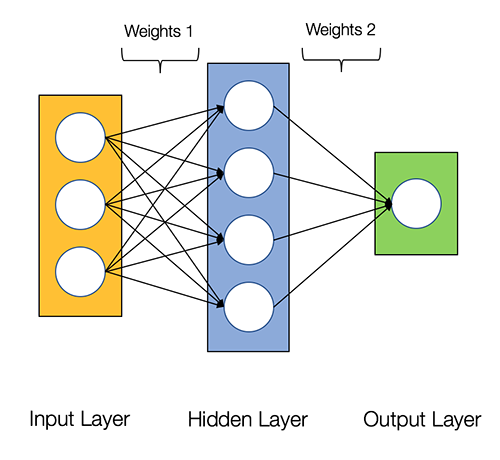
\includegraphics[width=\textwidth]{1.png}

用Python可以很容易的构建神经网络类

\begin{lstlisting}[language=python, breaklines]
class NeuralNetwork:
    def __init__(self, x, y):
        self.input      = x
        self.weights1   = np.random.rand(self.input.shape[1],4) 
        self.weights2   = np.random.rand(4,1)                 
        self.y          = y
        self.output     = np.zeros(y.shape)
\end{lstlisting}

\subsection{训练神经网络}

这个网络的输出$\hat{y}$为:

\begin{equation}
    \hat{y} = \sigma (W_2 \sigma (W_1 x + b_1) + b_2)
\end{equation}

你可能会注意到,在上面的等式中,输出$\hat{y}$是$W$和$b$函数。

因此$W$和$b$的值影响预测的准确率. 所以根据输入数据对$W$和$b$调优的过程就被成为训练神经网络。

每步训练迭代包含以下两个部分:

\begin{itemize}
    \item 计算预测结果$\hat{y}$,这一步称为\textbf{前向传播}。
    \item 更新$W$和$b$,这一步称为\textbf{反向传播}。
\end{itemize}

下面的顺序图展示了这个过程:

\noindent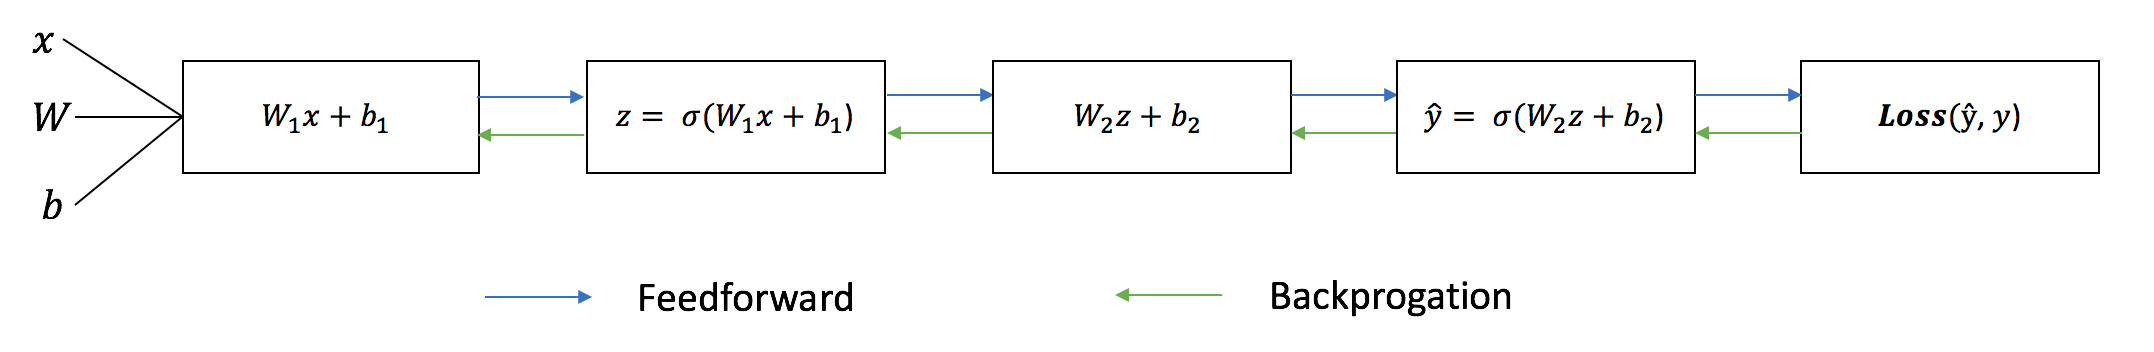
\includegraphics[width=\textwidth]{2.png}

\subsection{前向传播}

正如我们在上图中看到的,前向传播只是简单的计算。对于一个基本的2层网络来说,它的输出是这样的:

\begin{equation}
    \hat{y} = \sigma (W_2 \sigma (W_1 x + b_1) + b_2)
\end{equation}

我们在NeuralNetwork类中增加一个计算前向传播的函数。为了简单起见我们假设偏置$b$为$0$:

\begin{lstlisting}[language=python, breaklines]
class NeuralNetwork:
    def __init__(self, x, y):
        self.input      = x
        self.weights1   = np.random.rand(self.input.shape[1],4) 
        self.weights2   = np.random.rand(4,1)                 
        self.y          = y
        self.output     = np.zeros(self.y.shape)

    def feedforward(self):
        self.layer1 = sigmoid(np.dot(self.input, self.weights1))
        self.output = sigmoid(np.dot(self.layer1, self.weights2))
\end{lstlisting}

但是我们还需要一个方法来评估预测结果的好坏(即预测值和真实值的误差)。这就要用到损失函数。

\subsection{损失函数}

常用的损失函数有很多种,根据模型的需求来选择。在本教程中,我们使用误差平方和作为损失函数。

\begin{equation}
    Sum\text{--}of\text{--}Squares \ Error = \sum_{i=1}^{n}(y-\hat{y})^2.
\end{equation}

误差平方和是求每个预测值和真实值之间的误差再求和,这个误差是他们的差值求平方以便我们观察误差的绝对值。

训练的目标是找到一组$W$和$b$,使得损失函数最好小,也即预测值和真实值之间的距离最小。

\subsection{反向传播}

我们已经度量出了预测的误差(损失),现在需要找到一种方法来传播误差,并以此更新权值和偏置。

为了知道如何适当的调整权值和偏置,我们需要知道损失函数对权值$W$和偏置$b$的导数。

回想微积分中的概念,函数的导数就是函数的斜率。

\noindent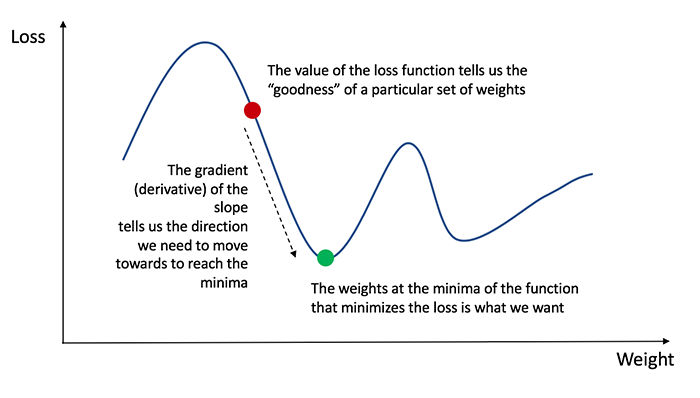
\includegraphics[width=\textwidth]{3.png}

如果我们已经求出了导数,我们就可以通过增加或减少导数值来更新权值$W$和偏置$b$(参考上图)。这种方式被称为梯度下降法。

但是我们不能直接计算损失函数对权值和偏置的导数,因为在损失函数的等式中并没有显式的包含他们。因此,我们需要运用链式求导发在来帮助计算导数。

\begin{equation}
    Loss(y,\hat{y})=\sum_{i=1}^{n}(y-\hat{y})^2
\end{equation}

\begin{equation}
    \begin{split}
        \frac{\partial Loss(y,\hat{y})}{\partial W} &= 
        \frac{\partial Loss(y,\hat{y})}{\partial \hat{y}} * \frac{\partial \hat{y}}{\partial z} * \frac{\partial z}{\partial W} \quad where \quad z = Wx + b \\
        &= 2(y-\hat{y})*Sigmoid \text{函数的导数}*x \\
        &= 2(y-\hat{y})*z(1-z)*x
    \end{split}
\end{equation}

链式法则用于计算损失函数对$W$和$b$的导数。注意,为了简单起见。我们只展示了假设网络只有$1$层的偏导数。

这虽然很简陋,但是我们依然能得到想要的结果—损失函数对权值$W$的导数(斜率),因此我们可以相应的调整权值。

现在我们将反向传播算法的函数添加到Python代码中

\begin{lstlisting}[language=python, breaklines]
class NeuralNetwork:
    def __init__(self, x, y):
        self.input      = x
        self.weights1   = np.random.rand(self.input.shape[1],4) 
        self.weights2   = np.random.rand(4,1)                 
        self.y          = y
        self.output     = np.zeros(self.y.shape)

    def feedforward(self):
        self.layer1 = sigmoid(np.dot(self.input, self.weights1))
        self.output = sigmoid(np.dot(self.layer1, self.weights2))

    def backprop(self):
        # application of the chain rule to find derivative of the loss function with respect to weights2 and weights1
        d_weights2 = np.dot(self.layer1.T, (2*(self.y - self.output) * sigmoid_derivative(self.output)))
        d_weights1 = np.dot(self.input.T,  (np.dot(2*(self.y - self.output) * sigmoid_derivative(self.output), self.weights2.T) * sigmoid_derivative(self.layer1)))

        # update the weights with the derivative (slope) of the loss function
        # 利用求得的梯度更新权值,所以叫梯度下降
        self.weights1 += d_weights1
        self.weights2 += d_weights2
\end{lstlisting}

\section{整合并完成一个实例}

既然我们已经有了包括前向传播和反向传播的完整Python代码,那么就将其应用到一个例子上看看它是如何工作的吧。

\noindent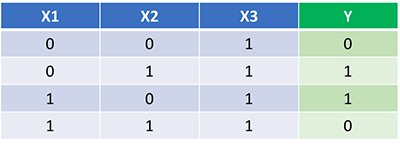
\includegraphics[width=\textwidth]{4.png}

神经网络可以通过学习得到函数的权重。而我们仅靠观察是不太可能得到函数的权重的。

让我们训练神经网络进行1500次迭代,看看会发生什么。 注意观察下面每次迭代的损失函数,我们可以清楚地看到损失函数单调递减到最小值。这与我们之前介绍的梯度下降法一致。

\noindent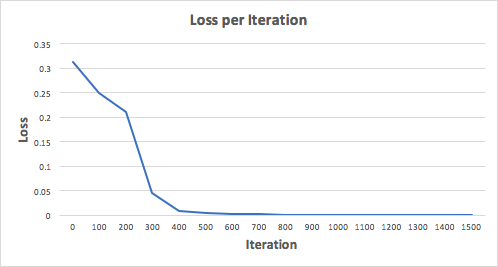
\includegraphics[width=\textwidth]{5.png}

让我们看看经过1500次迭代后的神经网络的最终预测结果:

\noindent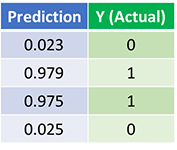
\includegraphics[width=\textwidth]{6.png}

经过1500次迭代训练后的预测结果

我们成功了!我们应用前向和方向传播算法成功的训练了神经网络并且预测结果收敛于真实值。

注意预测值和真实值之间存在细微的误差是允许的。这样可以防止模型过拟合并且使得神经网络对于未知数据有着更强的泛化能力。

\section{下一步是什么?}

幸运的是我们的学习之旅还没有结束,仍然有很多关于神经网络和深度学习的内容需要学习。例如:

\begin{itemize}
    \item 除了Sigmoid以外,还可以用哪些激活函数
    \item 在训练网络的时候应用学习率
    \item 在面对图像分类任务的时候使用卷积神经网络
\end{itemize}

我很快会写更多关于这个主题的内容,敬请期待!

\section{最后的想法}

我自己也从零开始写了很多神经网络的代码。

虽然可以使用诸如Tensorflow和Keras这样的深度学习框架方便的搭建深层网络而不需要完全理解其内部工作原理。但是我觉得对于有追求的数据科学家来说,理解内部原理是非常有益的。

这种练习对我自己来说已成成为重要的时间投入,希望也能对你有所帮助。

\section{推导笔记}

这里要注意的一点是,程序中将偏置$b$设置为了$0$。所以预测结果为:

\begin{align*}
    \hat{y} = \sigma (W_2 \sigma(W_1 X)) \\
    layer1 = \sigma(W_1 X) \\
    output = \sigma(W_2 layer1)
\end{align*}

用到的矩阵求导的一个公式如下,假设$A$和$B$都是矩阵,则

\begin{equation}
    \frac{\partial AB}{A} = B^T
\end{equation}
\chapter{使用NumPy实现一个复杂的深度神经网络}

\section{导言}

在正式开始之前,需要先对所做实验进行构思。我们想要编写一个程序,使其能够创建一个具有指定架构(层的数量、大小以及激活函数)的神经网络,如下图所示。总之,我们需要预先对网络进行训练,然后利用它进行预测。

\noindent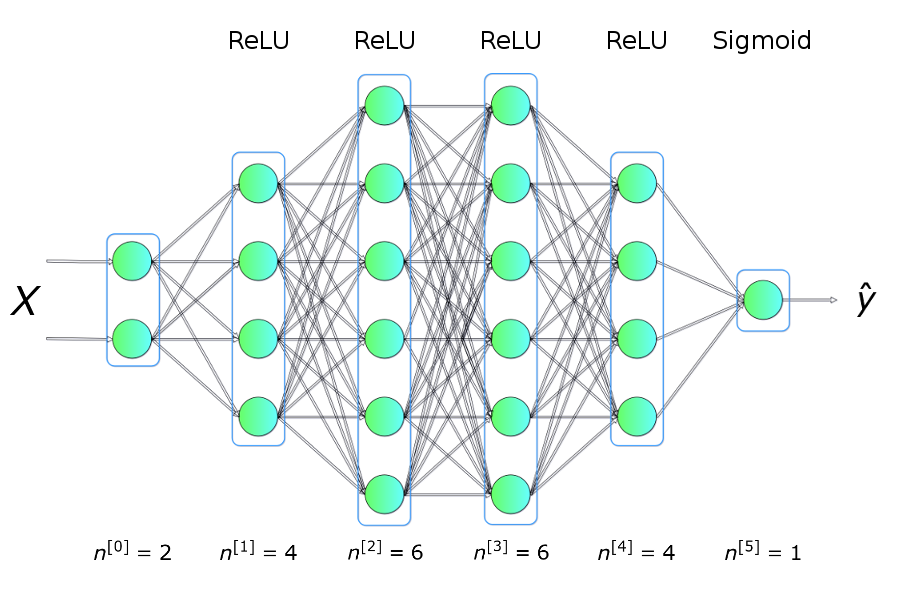
\includegraphics[width=\textwidth]{7.png}

\section{神经网络层的初始化}

首先,对每一层的权重矩阵$W$及偏置向量$b$进行初始化。在下图中,上标$[l]$表示目前是第几层(从$1$开始),$n$的值表示一层中的神经元数量。描述神经网络架构的信息类似于下面的代码片段中所列内容。每一项都描述了单层神经网络的基本参数:input\_dim,即输入层神经元维度;output\_dim,即输出层神经元维度;activation,即使用的激活函数。

\noindent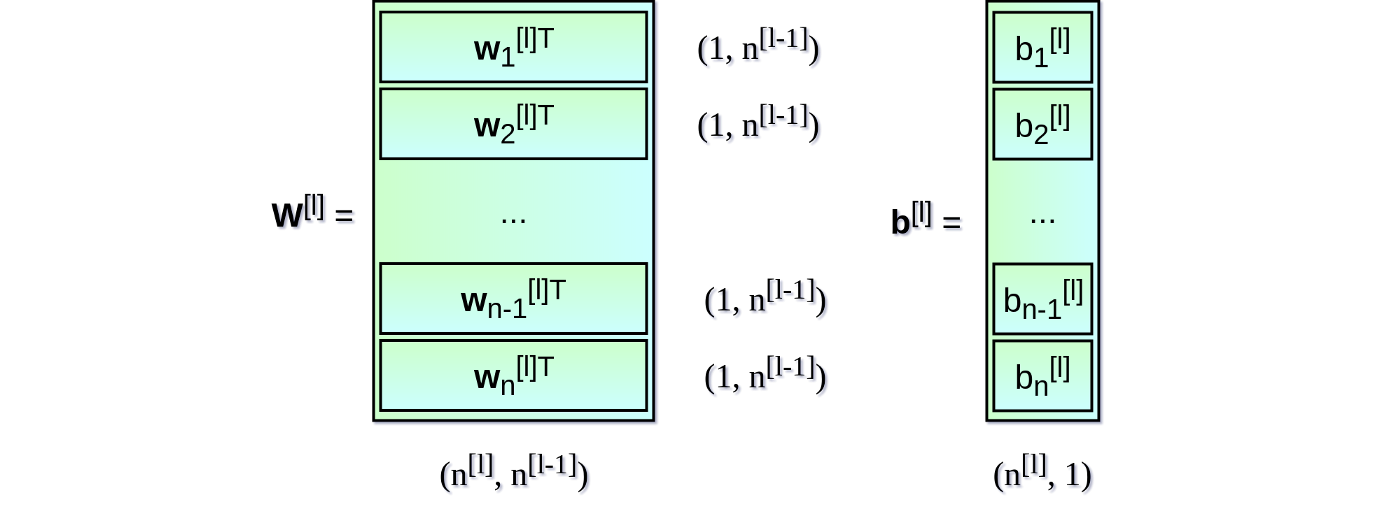
\includegraphics[width=\textwidth]{8.png}

代码片段如下:

\begin{lstlisting}[language=python, breaklines]
nn_architecture = [
    {"input_dim": 2, "output_dim": 4, "activation": "relu"},
    {"input_dim": 4, "output_dim": 6, "activation": "relu"},
    {"input_dim": 6, "output_dim": 6, "activation": "relu"},
    {"input_dim": 6, "output_dim": 4, "activation": "relu"},
    {"input_dim": 4, "output_dim": 1, "activation": "sigmoid"},
]
\end{lstlisting}

从上面的代码片段中可以看出,每一层输出神经元的维度等于下一层的输入维度。对权重矩阵W及偏置向量b进行初始化的代码如下:

\begin{lstlisting}[language=python, breaklines]
def init_layers(nn_architecture, seed = 99):
    np.random.seed(seed)
    number_of_layers = len(nn_architecture)
    params_values = {}

    for idx, layer in enumerate(nn_architecture):
        layer_idx = idx + 1
        layer_input_size = layer["input_dim"]
        layer_output_size = layer["output_dim"]
        
        params_values['W' + str(layer_idx)] = np.random.randn(
            layer_output_size, layer_input_size) * 0.1
        params_values['b' + str(layer_idx)] = np.random.randn(
            layer_output_size, 1) * 0.1
        
    return params_values
\end{lstlisting}

在本节中,我们利用NumPy将权重矩阵$W$及偏置向量$b$初始化为小的随机数。特别注意的是,初始化权重值不能相同,否则网络会变为对称的。也就是说,如果权重初始化为同一值,则对于任何输入$X$,每个隐藏层对应的每个神经元的输出都是相同的,这样即使梯度下降训练,无论训练多少次,这些神经元都是对称的,无论隐藏层内有多少个结点,都相当于在训练同一个函数。

初始化的值较小能够使得算法第一次迭代的时候效率更高。

\section{激活函数}

激活函数在神经网络中至关重要,其原理简单但功能强大,给神经元引入了非线性因素,使得神经网络可以任意逼近任何非线性函数,从而应用于众多的非线性模型。“如果没有激活函数,每一层输出都是上层输入的线性函数,无论神经网络有多少层,输出都是输入的线性组合。”激活函数种类众多,本文选取了最常用的两种——ReLU及Sigmoid函数,代码如下:

\begin{lstlisting}[language=python, breaklines]
def sigmoid(Z):
    return 1/(1+np.exp(-Z))

def relu(Z):
    return np.maximum(0,Z)

def sigmoid_backward(dA, Z):
    sig = sigmoid(Z)
    return dA * sig * (1 - sig)

def relu_backward(dA, Z):
    dZ = np.array(dA, copy = True)
    dZ[Z <= 0] = 0
    return dZ
\end{lstlisting}

\section{前向传播算法}

本文所设计的神经网络结构简单,信息流只有一个方向:以$X$矩阵的形式传递,穿过所有隐藏层单元,最终输出预测结构$\hat{Y}$。

\begin{lstlisting}[language=python, breaklines]
def single_layer_forward_propagation(A_prev, W_curr, b_curr, activation="relu"):
    Z_curr = np.dot(W_curr, A_prev) + b_curr
    
    if activation is "relu":
        activation_func = relu
    elif activation is "sigmoid":
        activation_func = sigmoid
    else:
        raise Exception('Non-supported activation function')
        
    return activation_func(Z_curr), Z_curr
\end{lstlisting}

前向传播就是上层处理完的数据作为下一层的输入数据,然后进行处理(权重),再传给下一层,这样逐层处理,最后输出。给定上一层的输入信号,计算仿射变换(affine transformation)Z,然后应用选定的激活函数。

前向传播算法代码如下,该函数不仅进行预测计算,还存储中间层A和Z矩阵的值:

\begin{lstlisting}[language=python, breaklines]
def full_forward_propagation(X, params_values, nn_architecture):
    memory = {}
    A_curr = X
    
    for idx, layer in enumerate(nn_architecture):
        layer_idx = idx + 1
        A_prev = A_curr
        
        activ_function_curr = layer["activation"]
        W_curr = params_values["W" + str(layer_idx)]
        b_curr = params_values["b" + str(layer_idx)]
        A_curr, Z_curr = single_layer_forward_propagation(A_prev, W_curr, b_curr, activ_function_curr)
        
        memory["A" + str(idx)] = A_prev
        memory["Z" + str(layer_idx)] = Z_curr
       
    return A_curr, memory
\end{lstlisting}

\section{损失函数}

损失函数是用来估量模型的预测值与真实值的不一致程度,它是一个非负实值函数。损失函数由我们想要解决的问题所决定。在本文中,我们想要测试神经网络模型区分两个类别的能力,所以选择了交叉熵损失函数,其定义如下:

\begin{align*}
    J(W, b) = \frac{1}{m}\sum_{i=1}^m L(\hat{y}^{(i)},y^{(i)}) \\
    L(\hat{y},y)=-(y\log \hat{y} + (1-y)\log(1-\hat{y}))
\end{align*}

为了更加清楚的了解学习过程,我增添了一个用于计算精度的函数:

\begin{lstlisting}[language=python, breaklines]
def get_cost_value(Y_hat, Y):
    m = Y_hat.shape[1]
    cost = -1 / m * (np.dot(Y, np.log(Y_hat).T) + np.dot(1 - Y, np.log(1 - Y_hat).T))
    return np.squeeze(cost)

def get_accuracy_value(Y_hat, Y):
    Y_hat_ = convert_prob_into_class(Y_hat)
    return (Y_hat_ == Y).all(axis=0).mean()
\end{lstlisting}

\section{反向传播算法}

许多缺乏经验的深度学习爱好者认为反向传播是一种复杂且难以理解的算法。

\begin{lstlisting}[language=python, breaklines]
def single_layer_backward_propagation(dA_curr, W_curr, b_curr, Z_curr, A_prev, activation="relu"):
    m = A_prev.shape[1]
    
    if activation is "relu":
        backward_activation_func = relu_backward
    elif activation is "sigmoid":
        backward_activation_func = sigmoid_backward
    else:
        raise Exception('不支持的激活函数')
    
    dZ_curr = backward_activation_func(dA_curr, Z_curr)
    dW_curr = np.dot(dZ_curr, A_prev.T) / m
    db_curr = np.sum(dZ_curr, axis=1, keepdims=True) / m
    dA_prev = np.dot(W_curr.T, dZ_curr)

    return dA_prev, dW_curr, db_curr
\end{lstlisting}

其实,他们困惑的也就是反向传播算法中的梯度下降问题,但二者并不可混为一谈。前者旨在有效地计算梯度,而后者是利用计算得到的梯度进行优化。梯度下降可以应对带有明确求导函数的情况,我们可以把它看作没有隐藏层的网络;但对于多隐藏层的神经网络,应先将误差反向传播至隐藏层,然后再应用梯度下降,其中将误差从最末层往前传递的过程需要链式法则,反向传播算法可以说是梯度下降在链式法则中的应用。对于单层的神经网络,该过程如下所示:

\begin{align*}
    \mathbf{dW}^{[l]} = \frac{\partial L}{\partial \mathbf{W}^{[l]}} = \frac{1}{m}\mathbf{dZ}^{[l]}\mathbf{A}^{[l-1]T} \\
    \mathbf{db}^{[l]} = \frac{\partial L}{\partial \mathbf{b}^{[l]}} = \frac{1}{m}\sum_{i=1}^m\mathbf{dZ}^{[l](i)} \\
    \mathbf{dA}^{[l-1]}=\frac{\partial L}{\partial \mathbf{A}^{[l]}} * g'(\mathbf(Z)^{[l]})
\end{align*}

本文省略推导过程,但从上面的公式仍可看出$A$和$Z$矩阵值的重要性。

上面的代码中所示代码仅编写了神经网络中某层的反向传播算法,下面的代码将展示神经网络中完整的反向传播算法。

\begin{lstlisting}[language=python, breaklines]
def full_backward_propagation(Y_hat, Y, memory, params_values, nn_architecture):
    grads_values = {}
    m = Y.shape[1]
    Y = Y.reshape(Y_hat.shape)
   
    dA_prev = - (np.divide(Y, Y_hat) - np.divide(1 - Y, 1 - Y_hat));
    
    for layer_idx_prev, layer in reversed(list(enumerate(nn_architecture))):
        layer_idx_curr = layer_idx_prev + 1
        activ_function_curr = layer["activation"]
        
        dA_curr = dA_prev
        
        A_prev = memory["A" + str(layer_idx_prev)]
        Z_curr = memory["Z" + str(layer_idx_curr)]
        W_curr = params_values["W" + str(layer_idx_curr)]
        b_curr = params_values["b" + str(layer_idx_curr)]
        
        dA_prev, dW_curr, db_curr = single_layer_backward_propagation(
            dA_curr, W_curr, b_curr, Z_curr, A_prev, activ_function_curr)
        
        grads_values["dW" + str(layer_idx_curr)] = dW_curr
        grads_values["db" + str(layer_idx_curr)] = db_curr
    
    return grads_values    
\end{lstlisting}

\section{参数更新}

该部分旨在利用计算得到梯度更新网络中的参数,同时最小化目标函数。我们会使用到params\_values,它存放当前的参数值,以及grads\_values,它存放存储关于这些参数的损失函数的导数。现在只需要在神经网络的每层应用如下公式即可:

\begin{align*}
\mathbf{W}^{[l]} = \mathbf{W}^{[l]} - \alpha\mathbf{dW}^{[l]} \\
\mathbf{b}^{[l]} = \mathbf{b}^{[l]} - \alpha\mathbf{db}^{[l]}
\end{align*}

代码片段如下:

\begin{lstlisting}
def update(params_values, grads_values, nn_architecture, learning_rate):
    for layer_idx, layer in enumerate(nn_architecture):
        params_values["W" + str(layer_idx)] -= learning_rate * grads_values["dW" + str(layer_idx)]        
        params_values["b" + str(layer_idx)] -= learning_rate * grads_values["db" + str(layer_idx)]

    return params_values;
\end{lstlisting}

\section{整合}

现在我们只需将准备好的函数按照正确的顺序整合到一起,若对正确的顺序有疑问请参见图2。

\begin{lstlisting}
def train(X, Y, nn_architecture, epochs, learning_rate):
    params_values = init_layers(nn_architecture, 2)
    cost_history = []
    accuracy_history = []
    
    for i in range(epochs):
        Y_hat, cashe = full_forward_propagation(X, params_values, nn_architecture)
        cost = get_cost_value(Y_hat, Y)
        cost_history.append(cost)
        accuracy = get_accuracy_value(Y_hat, Y)
        accuracy_history.append(accuracy)
        
        grads_values = full_backward_propagation(Y_hat, Y, cashe, params_values, nn_architecture)
        params_values = update(params_values, grads_values, nn_architecture, learning_rate)
        
    return params_values, cost_history, accuracy_history    
\end{lstlisting}

\section{对比分析}

接下来,我们将利用所构建的模型解决简单的分类问题。如图7所示,本次实验使用的数据集包含两个类别。我们将训练模型对两个不同的类别进行区分。此外,我们还准备了一个由Keras所构建的神经网络模型以进行对比。两个模型具有相同的架构和学习速率。虽然我们的模型很简单,但结果表明,NumPy和Keras模型在测试集上均达到了95\%的准确率。只是我们的模型耗费了更多的时间,未来工作可通过加强优化改善时间开销问题。
    
\end{document}